%% 
%% Copyright 2019-2021 Elsevier Ltd
%% 
%% This file is part of the 'CAS Bundle'.
%% --------------------------------------
%% 
%% It may be distributed under the conditions of the LaTeX Project Public
%% License, either version 1.2 of this license or (at your option) any
%% later version.  The latest version of this license is in
%%    http://www.latex-project.org/lppl.txt
%% and version 1.2 or later is part of all distributions of LaTeX
%% version 1999/12/01 or later.
%% 
%% The list of all files belonging to the 'CAS Bundle' is
%% given in the file `manifest.txt'.
%% 
%% Template article for cas-sc documentclass for 
%% single column output.

\documentclass[a4paper,fleqnn]{cas-sc}

% If the frontmatter runs over more than one page
% use the longmktitle option.

%\documentclass[a4paper,fleqn,longmktitle]{cas-sc}

\hypersetup{colorlinks=true,allcolors=cyan}
%\usepackage[numbers]{natbib}
\usepackage[authoryear]{natbib}
%\usepackage[authoryear,longnamesfirst]{natbib}


%Cuong
\usepackage{amssymb}
\usepackage{latexsym}
\usepackage{amsmath}
\usepackage{dsfont}
\usepackage{amsfonts}
\usepackage{bigdelim}
%\usepackage[section]{placeins}
\usepackage{graphicx}
\usepackage{caption}
\usepackage{subcaption}
\captionsetup[subfloat]{labelformat=empty, font=footnotesize}
\usepackage{float}

%%%Author macros
\def\tsc#1{\csdef{#1}{\textsc{\lowercase{#1}}\xspace}}
\tsc{WGM}
\tsc{QE}
%%%

% Uncomment and use as if needed
%\newtheorem{theorem}{Theorem}
%\newtheorem{lemma}[theorem]{Lemma}
%\newdefinition{rmk}{Remark}
%\newproof{pf}{Proof}
%\newproof{pot}{Proof of Theorem \ref{thm}}

\begin{document}
\let\WriteBookmarks\relax
\def\floatpagepagefraction{1}
\def\textpagefraction{.001}

% Short title
\shorttitle{}    

% Main title of the paper
\title [mode = title]{Vote-based RGBD Fusion for Hand-held Object Pose Estimation}  

% Title footnote mark
% eg: \tnotemark[1]
%\tnotemark[1] 

% Title footnote 1.
% eg: \tnotetext[1]{Title footnote text}
%\tnotetext[1]{tnote text} 

% First author
%
% Options: Use if required
% eg: \author[1,3]{Author Name}[type=editor,
%       style=chinese,
%       auid=000,
%       bioid=1,
%       prefix=Sir,
%       orcid=0000-0000-0000-0000,
%       facebook=<facebook id>,
%       twitter=<twitter id>,
%       linkedin=<linkedin id>,
%       gplus=<gplus id>]


% Footnote text
%\fntext[1]{}

% For a title note without a number/mark
%\nonumnote{}

% Here goes the abstract
\begin{abstract}
Estimating the 6D pose of objects in hand is a challenging and critical problem in computer vision and robotics, particularly for applications like robotic manipulation, human-robot interaction, and augmented reality (AR). Leveraging multi-modal data, such as color (RGB) and depth (D) images, offers a promising approach. Despite significant progress in representation learning across these modalities, this field faces two major issues. First, the presence of a hand often causes significant occlusions, which conventional object pose estimation methods struggle to handle effectively. Second, existing approaches typically extract features from two separate backbones and fuse the data at the feature level. This fusion mechanism can cause a representation distribution shift and potential disruption during fine-tuning due to dense interactions between the RGB and depth branches. In this work, we propose a novel deep neural network for hand-held object pose estimation using an RGB-D image as input. Instead of fusing data at the feature level, we introduce a vote-based fusion mechanism to effectively combine multimodal data for the pose estimation task, particularly for occluded objects in the presence of a hand. Additionally, we model the relationship between the hand and the object through keypoint interaction, incorporating this relationship into the object pose estimation process. Through experiments on three public datasets, our approach demonstrates significant improvements in accuracy and robustness over existing methods, achieving an accuracy improvement of up to 15\%.
\end{abstract}

% Use if graphical abstract is present
%\begin{graphicalabstract}
%\includegraphics{}
%\end{graphicalabstract}

% Research highlights
%\begin{highlights}
%\item 
%\item 
%\item 
%\end{highlights}

% Keywords
% Each keyword is seperated by \sep
\begin{keywords}
 \sep Object pose estimation \sep Object recognition \sep Multimodal fusion \sep
\end{keywords}

\maketitle

%%%%%%%%%%%%%%%%%%%%%%%%%%%%%%%%%%%%%%%%%%%%%%%%%%%%%%%%%%%%%%%%%%%%%%

\section{Introduction}
\label{sec:intro}

Estimating the 6D pose of hand-held objects is an important yet challenging task in robotics (\cite{pfanne2018fusing, anzai2020deep, okafor2024deep}), virtual reality \cite{muhanna2015virtual}, among others. It plays a significant role in applications such as robotic manipulation or human-robot interaction (\cite{andrychowicz2020learning, handa2020dexpilot}). The increasing availability of 3D sensors has made RGB-D data more accessible, which, when incorporating 3D geometric information from depth sensors, allows for more accurate and robust 6D pose estimation compared to using RGB data alone. However, despite notable advancements in multi-modal representation learning, significant challenges remain. These challenges are primarily due to occlusions caused by the hand and the complexities involved in effectively fusing RGB and depth data (\cite{chao2021dexycb}). Traditional methods (\cite{wang20216d, peng2019pvnet, wang2019densefusion, sharma2022saliency}) struggle with accuracy drops when hands occlude objects, as hands obscure critical features needed for precise pose estimation. These occlusions introduce ambiguities and complexities, making it difficult to determine the object's orientation and position. Some approaches attempt to segment the hand or predict occluded regions, but these add complexity and often fall short under challenging conditions (\cite{he2020pvn3d, castro2023crt}). Additionally, hand-object interactions introduce non-rigid transformations, further complicating pose estimation by distorting the object's perceived shape and pose due to varying grips and manipulations.

Current mainstream RGBD fusion methods typically employ separate RGB pre-trained backbones to extract features from RGB images and depth maps (\cite{wang2019densefusion, he2020pvn3d, he2021ffb6d}). These backbones independently extract features from their respective modalities, which are then integrated during subsequent processing stages. Despite achieving high performance on benchmark datasets, several critical issues persist. The RGBD backbones are designed to handle input as image-depth pairs, which contrasts with the single-image input used in RGB pretraining. This difference often leads to a significant shift in representation distribution. Specifically, the features learned from single RGB images may not directly align with those extracted from RGBD inputs, impacting the model's ability to generalize effectively across both modalities. Moreover, during fine-tuning, extensive interactions occur between the RGB and depth branches. These interactions are crucial for integrating complementary information from both sources. However, the dense coupling between these branches can potentially disturb the original representation distribution learned by the pretrained RGB backbone. This phenomenon may hinder the model's capacity to leverage the full potential of the RGB features, thereby affecting overall performance and generalization ability on RGBD tasks.

In this paper, we present a novel deep neural network specifically designed for hand-held object pose estimation using RGB-D images. Different from traditional feature-level fusion methods, our approach introduces a vote-based fusion mechanism that effectively integrates multimodal data. This mechanism leverages a voting scheme where both 2D and 3D keypoints cast votes for the object's pose, particularly enhancing the estimation in scenarios with occluded objects. By combining votes from different modalities, our method mitigates the issues of representation distribution shift and potential disruptions during fine-tuning, leading to more accurate pose predictions. Furthermore, we model the interaction between the hand and the object through self-attention mechanism, integrating this relationship into the pose estimation process. Our network predicts keypoints for both the hand and the object, using these keypoints to establish a contextual relationship that enhances the pose estimation, especially when the object is partially obscured by the hand. This hand-object keypoint interaction modeling allows our method to account for non-rigid transformations and occlusions introduced by the hand, significantly improving the robustness of the pose estimation.

The primary contributions of this work can be summarized as follows:

\begin{itemize}

\item \textbf{Vote-based Fusion Module} $\mathcal{M}_{fus}$: We introduce a vote-based fusion mechanism that integrates RGB and depth data more effectively than traditional feature-level fusion methods. This module utilizes both 2D and 3D features, leveraging a radius-based neighborhood projection and channel attention mechanisms to enhance the representation of crucial features while mitigating noise and redundancy. \\

\item \textbf{Hand-aware Object Pose Estimation Module} $\mathcal{M}_{hao}$: By modeling the relationship between the hand and the object through a self-attention mechanism, we enhance the pose estimation process. This self-attention mechanism captures complex spatial relationships between keypoints, which is crucial for accurately estimating the pose of objects that are partially occluded by the hand.

\item \textbf{Comprehensive Experimental Validation}: We provide extensive experimental validation across three public datasets: DexYCB (\cite{chao2021dexycb}), FPHAB (\cite{garcia2018first}), and HO-3D (\cite{hampali2020honnotate}). Our method consistently outperforms state-of-the-art approaches, achieving significant improvements in all metrics. Additionally, our method achieves competitive inference times, making it suitable for real-world applications. \\

\end{itemize} 
%
\section{Related work}
\label{sec:relatedwork}

\subsection{Object Pose Estimation From Visual Inputs}

Object pose estimation is a well-explored field in computer vision, focusing on determining the position and orientation (pose) of objects from visual inputs such as RGB or depth images \cite{wang2019densefusion, he2020pvn3d, he2021ffb6d}. Deep learning-based methods have significantly advanced pose estimation by learning rich feature representations directly from the data \cite{wang2021gdr, peng2019pvnet}. These methods can be broadly categorized into two main types: depth-based methods, RGB-based methods, RGBD-based methods. Depth-based object pose estimation uses depth sensors to capture the 3D structure of objects, extracting geometric information from depth maps \cite{wang20216d, gao20206d, guo2021efficient}. This approach is beneficial in low-light conditions or when RGB-based methods fail due to insufficient texture. However, depth sensors can produce noisy or incomplete data, especially with occlusions or reflective surfaces, and processing dense point clouds can be computationally expensive for real-time applications. RGB-based methods estimate object poses using color images, leveraging texture and color information to identify and localize objects \cite{billings2019silhonet, peng2019pvnet, wang2021gdr}. Common techniques include keypoint detection, feature matching, and deep learning-based regression. These methods perform well in well-lit environments with distinct textures but struggle with varying lighting conditions and occlusions. They are also less effective for objects with uniform or repetitive textures, where the lack of distinct features makes pose estimation challenging. 

RGBD-based methods combine the strengths of both RGB and depth-based approaches by leveraging multimodal data \cite{wang2019densefusion, he2020pvn3d, hong2024rdpn6d}. These methods utilize both color and depth information to provide a more comprehensive understanding of the object's geometry and appearance. By integrating RGB and depth data, RGBD-based methods can achieve higher accuracy and robustness in pose estimation. Existing data fusion methods often involve combining features from RGB and depth modalities at various stages of the neural network. Common approaches include early fusion (combining raw data), middle fusion (combining intermediate features), and late fusion (combining final predictions). Each method has its advantages and drawbacks. Early fusion can lead to high-dimensional inputs and increased computational costs, while late fusion may miss out on capturing interactions between modalities during feature extraction. Middle fusion strikes a balance but can still suffer from representation distribution shifts. In hand-held object pose estimation, the presence of the hand introduces non-rigid transformations and occlusions that further complicate the fusion process. Existing methods may not effectively model the interaction between the hand and the object, leading to reduced accuracy in pose estimation. In this work, we propose a novel deep neural network for hand-held object pose estimation using an RGB-D image as input. Instead of fusing data at the feature level, we introduce a vote-based fusion mechanism to effectively combine multimodal data for the pose estimation task, particularly for occluded objects in the presence of a hand. 

\subsection{Voting Mechanism In Visual Tasks}

Voting mechanisms have been widely used in computer vision tasks to enhance robustness and accuracy. These mechanisms involve aggregating multiple hypotheses or predictions to arrive at a consensus, which is particularly useful in noisy or ambiguous scenarios. The use of voting in visual tasks can be traced back to classical techniques like the Hough Transform, which aggregates votes in a parameter space to detect shapes in images \cite{hough1959machine}. In recent years, voting mechanisms have been integrated into deep learning frameworks to improve tasks such as object detection or pose estimation. VoteNet \cite{qi2019deep}, for instance, employs a voting scheme where 3D points cast votes for object centers, leading to robust object detection in point clouds. Inspired by this, Xie et al. \cite{xie2021venet} developed an enhanced VoteNet-based detector for cluttered indoor scenes, replacing the traditional MLP with an Attentive MLP (AMLP) for better feature description. Further, Mlcvnet \cite{xie2020mlcvnet} introduced Multi-Level Context VoteNet (MLCVNet), integrating context modules into voting and classification to encode contextual information at multiple levels. These include the Patch-to-Patch Context (PPC) for point patches, Object-to-Object Context (OOC) for object candidates, and Global Scene Context (GSC) for the overall scene. In RGB object pose estimation, voting mechanisms have proven highly effective. Peng et al. \cite{peng2019pvnet} introduced PVNet, which uses pixel-wise vector regression to vote for keypoint locations, aiding in the localization of occluded or truncated keypoints. He et al. \cite{he2020pvn3d} extended this by detecting 3D keypoints and estimating 6D pose parameters through a deep Hough voting network. Di et al. \cite{di2022gpv} later proposed GPV-Pose, which leverages geometric constraints for category-level pose estimation, using a 3D graph convolution encoder with branches for pose regression, symmetry-aware reconstruction, and point-wise bounding box voting.

Inspired by these successful implementations of voting mechanisms, we introduce a novel vote-based fusion mechanism for RGB-D images. Unlike existing methods that generate votes from depth images, RGB images, or fused RGB-D features, our approach separately performs voting in the 2D image branch and the 3D point cloud branch before combining the results. By leveraging both 2D and 3D keypoints, this method integrates multimodal data more effectively than traditional feature-level fusion methods, significantly enhancing pose estimation accuracy, especially in scenarios involving occluded objects.

%
\section{Methodology}
\label{sec:methodology}

\begin{figure*}[h!]
	\centering
	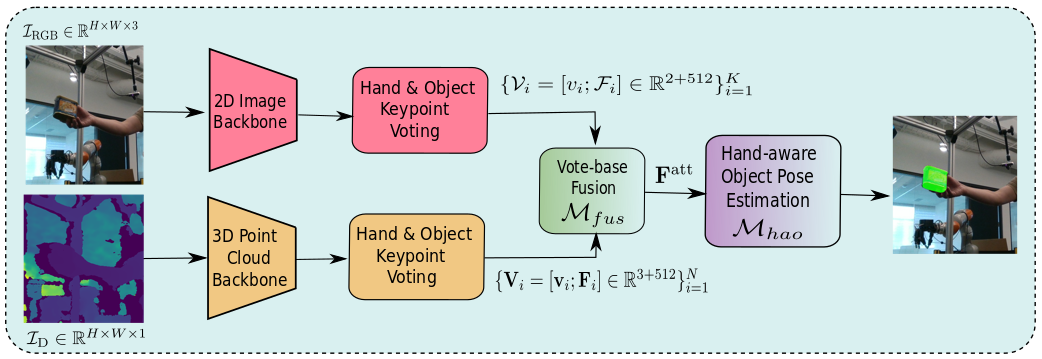
\includegraphics[width=0.98\linewidth]{figs/overview}
	\caption{Overview of our proposed framework for estimating the 6D pose of hand-held objects from RGB-D images. The framework comprises several key components: (1) feature extraction backbones for both 2D images and 3D point clouds, which process the RGB and depth information, respectively; (2) voting modules that generate votes for keypoint locations in both 2D and 3D spaces; (3) a vote-based fusion module $\mathcal{M}_{fus}$ that effectively combines the multimodal data to address the challenges of occlusions and representation distribution shifts; and (4) a hand-aware object pose estimation module $\mathcal{M}_{hao}$, which models the interactions between the hand and the object using a self-attention mechanism.}
	\label{fig:overview}
\end{figure*}

Our objective is to determine the 6D pose of a hand-held object within an RGB-D image. We assume the availability of an accurate 3D model of the object, with its coordinate system $\mathcal{O}$ defined in the model's 3D space. The pose of the object is described by a rigid transformation from the object coordinate system to the camera coordinate system $\mathcal{G}$. This transformation comprises a rotation matrix $R \in SO(3)$ and a translation vector $t \in \mathbb{R}^{3}$, collectively represented as $\xi = [R|t]$. Figure \ref{fig:overview} illustrates the overall pipeline of our framework. Our network consists of backbones for extracting features from both 2D images and 3D point clouds, voting modules, a vote-based fusion module $\mathcal{M}_{fus}$, and a hand-aware object pose estimation module $\mathcal{M}_{hao}$.

\subsection{3D Point Cloud Branch}

Given a depth image, the 3D point cloud branch network converts the image to a 3D point cloud and proceeds to cast votes for 3D keypoints of both hand and objects. Inspired by VoteNet (\cite{qi2019deep}), wherein 3D points participate in voting for object centers in object detection tasks, we have formulated our network to predict keypoint locations for individual 3D points. Specifically, we utilize the PointNet++ architecture (\cite{qi2017pointnet++}) with multi-scale grouping as our backbone network to extract geometric features. The backbone network takes $N$ points as input and enriches them with high-dimensional features $\{\mathbf{p}_{i}\}_{i=1}^{N}$ where $\mathbf{p}_{i} = [\mathbf{x}_i; \mathbf{f}_i]$ with $\mathbf{x}_{i}\in\mathbb{R}^{3}$ being the point location in 3D space and $\mathbf{f}_{i} \in \mathbb{R}^{512}$ being a feature vector.

Subsequently, the points $\{\mathbf{p}_{i}\}_{i=1}^{N}$ are fed into a multi-layer perceptron (MLP) to compute votes $\{\mathbf{V}_{i} = [\mathbf{v}_{i}; \mathbf{F}_{i}] \in \mathbb{R}^{3+512} \}_{i=1}^{N}$. The MLP consists of four fully connected layers, ReLU and batch normalization. Each vote $\mathbf{V}_i$ is represented by a point $\mathbf{v}_{i}$ in 3D space with its Euclidean coordinates supervised to be close to a keypoint $\mathbf{s}_i$, and a feature vector $\mathbf{F}_{i}$. To supervise the learning of votes $\{\mathbf{V}_{i} = [\mathbf{v}_{i}; \mathbf{F}_{i}] \in \mathbb{R}^{3+512} \}_{i=1}^{N}$, we apply a regression loss:

\begin{equation}
L_{\text{3d-vote}} = \dfrac{1}{N_{oh}} \sum_{i}  \| \mathbf{v}_{i} - \hat{\mathbf{v}}_{i} \|_{H} \cdot \mathds{1}(\mathbf{v}_{i})
\end{equation}

\noindent Here, $N_{oh}$ is the count of the total number of points on the object and hand, $\hat{\mathbf{v}}_{i}$ is the location of the closest ground truth keypoint, $\parallel\cdot\parallel_{H}$ is the Huber norm and $\mathds{1}(\cdot)$ is a binary function indicating whether the point $\mathbf{p}_i$ belongs to the hand or object. At this stage, we have a set of votes $\{\mathbf{V}_i = [\mathbf{v}_i; \mathbf{F}_i] \in \mathbb{R}^{3+512}\}_{i=1}^{N}$.

\subsection{2D Image Branch}

Given an input color image, this network branch predicts hand and object 2D keypoints. We adopt a pixel-wise direction prediction strategy, which encourages the network to prioritize local hand and object characteristics while minimizing the influence of cluttered backgrounds. We employ ResNet-34 (blocks 1, 2, 3, and 4) as the encoder, coupled with four up-sampling layers serving as the decoder (\cite{he2016deep}). The upsampling layers consist of transposed convolutional layers with batch normalization and ReLU activation. For a given pixel $p$, the network predicts a scale-invariant vector $\hat{\mathfrak{u}}(p)$, representing the direction from pixel $p$ to the closest keypoint $s$.

\begin{equation} 
\hat{\mathbf{u}}(p) = \frac{s - p}{\parallel s - p \parallel_2}
\end{equation}

\noindent To supervise the learning of unit vectors, we apply a smooth $L_1$ loss, similar to the approach in \cite{girshick2015fast}. The loss function $L_{\text{2d-vote}}$ is defined as:

\begin{equation} 
L_{\text{2d-vote}} = \dfrac{1}{N_{oh}} \sum_{p \in (\mathcal{O} \cup \mathcal{H})} \text{smooth}_{L_1} ( \hat{\mathbf{u}}(p) - \mathbf{u}(p) )
\end{equation}

\noindent Here, $N_{oh}$ is the count of the total number of pixels on the object and hand. $\mathbf{u}$ denotes the predicted vector, $\hat{\mathbf{u}}$ represents the ground truth unit vector, and $p \in (\mathcal{O} \cup \mathcal{H})$ indicates that pixel $p$ pertains to hand or object. Votes are generated by randomly selecting two pixels situated within a specific radius and then calculating the intersection of their respective vectors. Additionally, a representative feature is computed for these selected pixels through feature concatenation. This process is iterated $K$ times, leading to the generation of votes $\{ \mathcal{V}_{i} = [v_i; \mathcal{F}_i] \in \mathbb{R}^{2+512} \}_{i=1}^{K}$. $v_i \in \mathbb{R}^2$ represents the 2D vote location, and $\mathcal{F}_i \in \mathbb{R}^{512}$ represents the high-dimensional feature of the vote $v_i$.

\subsection{Vote-based Feature Fusion}

Given the votes \(\{\mathbf{V}_i = [\mathbf{v}_i; \mathbf{F}_i] \in \mathbb{R}^{3+512}\}_{i=1}^{N}\) from the 3D branch and \(\{\mathcal{V}_i = [v_i; \mathcal{F}_i] \in \mathbb{R}^{2+512}\}_{i=1}^{K}\) from the 2D branch, we perform vote-based fusion using a channel attention mechanism adapted for 3D data. For each geometric vote feature \(\mathbf{F}_i\) paired with its 3D point coordinate \(\mathbf{v}_i\), we retrieve the corresponding visual vote features from \(\mathcal{F}\) by projecting its neighborhood within a radius \(r\) onto the image plane. We then sample the \(k\) nearest neighbor votes within this region to gather their visual features. If fewer than \(k\) pixels exist in the corresponding region, null features are padded. The collected visual features are integrated using max pooling and processed through Multi-Layer Perceptrons (MLPs) to align their channel size with that of the point cloud features, producing modified visual vote features \(\mathcal{F}^{'}\):

\[
\mathcal{F}_i^{\text{proj}} = \text{MaxPool}(\{\mathcal{F}_j \mid \| v_j - \mathbf{v}_i \|_2 < r \})
\]

\[
\mathcal{F}_i^{'} = \text{MLP}_{\text{match}}(\mathcal{F}_i^{\text{proj}})
\]

\noindent Next, these integrated visual vote features \(\mathcal{F}_i^{'}\) are concatenated with the geometric vote features \(\mathbf{F}_i\), and a shared MLP is applied to produce fused vote features \(\{\mathbf{V}_i = [\mathbf{v}_i; \mathbf{F}_i^{\text{fus}}] \in \mathbb{R}^{3+1024}\}_{i=1}^{N}\):

\[
\mathbf{F}_i^{\text{fus}} = \text{MLP}_{\text{shared}}([\mathbf{F}_i; \mathcal{F}_i^{'}])
\]

\noindent To enhance these fused features, we employ a 3D channel attention module. This module uses global average pooling across all votes to generate a channel descriptor for each feature map. Specifically, global average pooling compresses each channel by computing the average of all values in that channel across all votes, resulting in a descriptor vector \(\mathbf{z}_c\):

\[
\mathbf{z}_c = \frac{1}{N} \sum_{i=1}^{N} \mathbf{F}^{\text{fus}}_i
\]

\noindent The channel descriptors are then passed through two fully connected layers to learn a weight vector. The first fully connected layer reduces the dimensionality, and the second fully connected layer restores it back to the original number of channels. Both layers use ReLU activations, except the final layer, which uses a sigmoid activation to normalize the weights between 0 and 1:

\[
\mathbf{w} = \sigma(\text{FC}_2(\text{ReLU}(\text{FC}_1(\mathbf{z}))))
\]

\noindent where \(\sigma\) denotes the sigmoid activation function. The learned weights are used to scale the channels of the fused feature map, effectively emphasizing the most informative channels and suppressing the less relevant ones:

\[
\mathbf{F}_i^{\text{att}} = \mathbf{w} \odot \mathbf{F}_i^{\text{fus}}
\]

\noindent where \(\odot\) denotes the Hadamard product (element-wise multiplication). This attention-enhanced fused feature, \(\mathbf{F}_i^{\text{att}}\), leverages both the geometric and visual information for improved hand-held object pose estimation. The channel attention mechanism recalibrates the features in each channel of the original feature points, enhancing the representation of more informative channels and suppressing less relevant ones. The design of this vote-based feature fusion is well-suited for RGB-D data fusion. By combining 2D and 3D features, we leverage the texture and color of RGB images with the spatial details of depth data. The radius-based neighborhood projection keeps the integration locally relevant, capturing necessary fine-grained details. Additionally, the channel attention mechanism enhances the fused features by prioritizing the most informative channels, reducing noise and redundancy, and dynamically adjusting each channel's contribution based on its relevance.

\subsection{Hand-aware Object Pose Estimation}

Given a set of votes $\{\mathbf{V}_i = [\mathbf{v}_i; \mathbf{F}_i^{\text{att}}] \in \mathbb{R}^{3+512}\}_{i=1}^{N}$, we sample a subset of $M$ votes (where $M < N$) using farthest point sampling based on $\{\mathbf{v}_i\}$ in 3D Euclidean space, to get $\{\mathbf{v}_i^m\}$ with $m = 1, \ldots, M$. Then we form $M$ clusters by finding neighboring votes to each of the $\mathbf{v}_i^m$'s 3D location:
\[
\mathbf{C}_m = \{\mathbf{V}_i \mid \|\mathbf{v}_i - \mathbf{v}_i^m\| \leq r\} \quad \text{for} \ m = 1, \ldots, M
\]
Here, $\mathbf{C}_m$ is the set of votes in the $m$-th cluster. Votes from each cluster are independently processed by $\text{MLP}_1$ before being max-pooled (channel-wise) to a single feature vector and passed to $\text{MLP}_2$ where information from different votes is further combined. Finally, each cluster yields a keypoint with a 3D position $\mathbf{x}_{j}^{\text{kp}} \in \mathbb{R}^{3}$ and an aggregated feature vector $F_{i} \in \mathbb{R}^{512}$. 

To better learn the relationship between the hand and the object, we integrate a self-attention module into the keypoint feature learning process. This module, inspired by the self-attention mechanism (\cite{zhang2019self}), encodes meaningful spatial relationships between the keypoints' features. Given the aggregated features $\{F_i \in \mathbb{R}^{512}\}_{i=1}^M$ from the $M$ keypoints, we apply the self-attention mechanism as follows. Firstly, the feature map $F_i$ is fed into two MLPs to generate two new feature maps $X$ and $Y$:
\[
X = \text{MLP}_1(F_i)
\]
\[
Y = \text{MLP}_2(F_i)
\]
Next, the attention map $W$ is computed as:
\[
W_{j,i} = \frac{\exp(Y_j \cdot X_i^T)}{\sum_{i=1}^{M} \exp(Y_j \cdot X_i^T)}
\]
where $W_{j,i}$ indicates that the $i$-th keypoint impacts the $j$-th keypoint. The original feature map $F_i$ is then fed into another MLP to output a new feature map $Z$:
\[
Z = \text{MLP}_3(F_i)
\]
We multiply $Z$ with the transpose of $W$ to generate the aggregated features $A^P$:
\[
A^P = W^T Z
\]
We then add a scale parameter $\mu$ and the original features to obtain the final enhanced feature map $F_i^{\text{att}}$:
\[
F_i^{\text{e}} = \mu A^P + F_i = \mu W^T Z + F_i
\]

This self-attention mechanism allows the network to learn the dependencies between different keypoints, capturing the complex relationships between the hand and the object, thus enhancing the feature representation for the hand-held object pose estimation. By incorporating this self-attention mechanism, the model can effectively leverage the spatial relationships between the keypoints to improve the accuracy and robustness of the pose estimation, leading to a more precise understanding of the hand-object interaction.

Given the enhanced keypoint features $\{\mathbf{F}_i^{\text{e}} \in \mathbb{R}^{512}\}_{i=1}^M$, we proceed to regress the object pose. Each enhanced feature $\mathbf{F}_i^{\text{e}}$ is input into an MLP-based regression network to predict the 3D object pose parameters. This regression network consists of several fully connected layers with ReLU activations, followed by an output layer that predicts the translation vector $\mathbf{t} \in \mathbb{R}^{3}$ and the rotation quaternion $\mathbf{q} \in \mathbb{R}^{4}$. The predicted pose $\{\mathbf{t}, \mathbf{q}\}$ represents the 3D translation and rotation of the object relative to the hand.

To train the network, we jointly supervise the learning of our modules using a multi-task loss function. This multi-task loss integrates several task-specific losses, each weighted by a respective factor, to ensure a balanced learning process across different aspects of pose estimation.

\begin{align}
L = L_{pose} + L_{3d-vote} + L_{2d-vote} + L_{sem}
\label{eq:loss}
\end{align}

\noindent Here, \(L\) represents the total loss, composed of the pose loss (\(L_{pose}\)), 3D voting loss (\(L_{3d-vote}\)), 2D voting loss (\(L_{2d-vote}\)), and semantic classification loss (\(L_{sem}\)). Following \cite{wang2019densefusion}, the pose loss is calculated as the distance between points sampled on the object model in the ground truth pose and the corresponding points transformed by the predicted pose. For symmetric objects, we minimize the distance from each point on the predicted model orientation to the nearest point on the ground truth model.
%
\section{Evaluation}
\label{sec:evaluation}

%--------------------------------------------------
\begin{figure*}[h!]
  \centering
  
  \begin{subfigure}[b]{0.16\linewidth}
    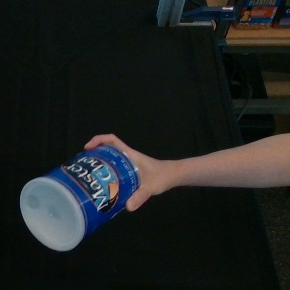
\includegraphics[width=0.98\linewidth]{figs/1000_rgb}
  \end{subfigure}
  \begin{subfigure}[b]{0.16\linewidth}
    
\includegraphics[width=0.98\linewidth]{figs/1000_depth2}
  \end{subfigure}
  \begin{subfigure}[b]{0.16\linewidth}
    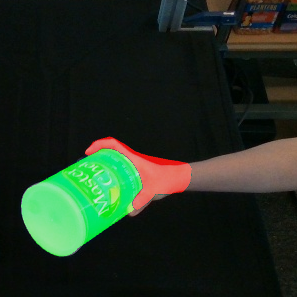
\includegraphics[width=0.98\linewidth]{figs/1000_0}
  \end{subfigure}
  \begin{subfigure}[b]{0.16\linewidth}
    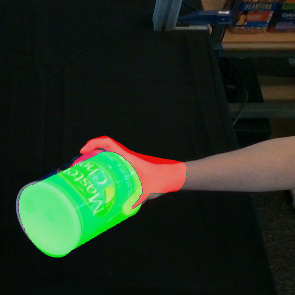
\includegraphics[width=0.98\linewidth]{figs/1000_4}
  \end{subfigure}
    \begin{subfigure}[b]{0.16\linewidth}
    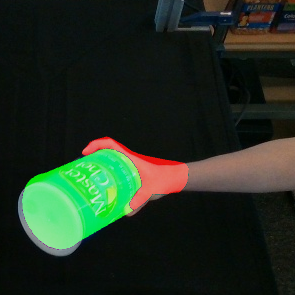
\includegraphics[width=0.98\linewidth]{figs/1000_5}
  \end{subfigure}
    \begin{subfigure}[b]{0.16\linewidth}
    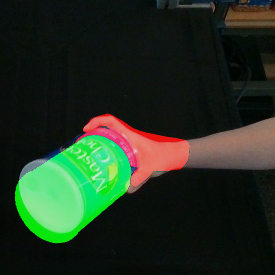
\includegraphics[width=0.98\linewidth]{figs/1000_8}
  \end{subfigure}  
  \vspace{0.2cm}
  
    \begin{subfigure}[b]{0.16\linewidth}
    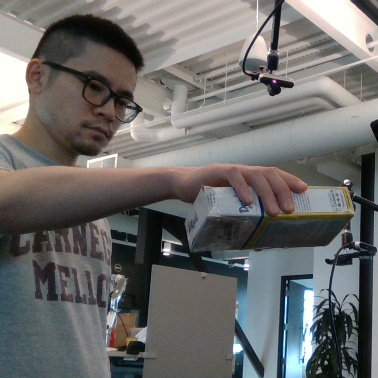
\includegraphics[width=0.98\linewidth]{figs/5319_rgb}
  \end{subfigure}
  \begin{subfigure}[b]{0.16\linewidth}
    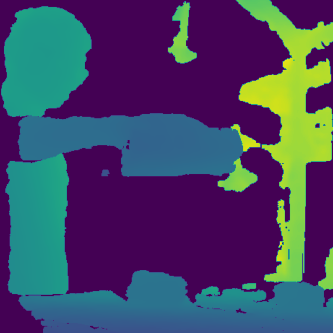
\includegraphics[width=0.98\linewidth]{figs/5319_depth2}
  \end{subfigure}
  \begin{subfigure}[b]{0.16\linewidth}
    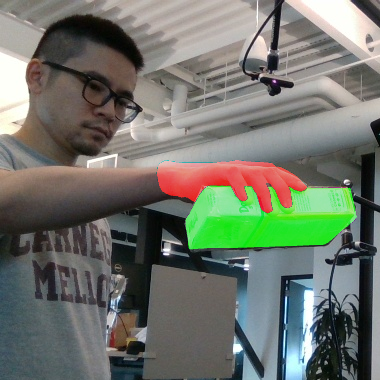
\includegraphics[width=0.98\linewidth]{figs/5319_1}
  \end{subfigure}
  \begin{subfigure}[b]{0.16\linewidth}
    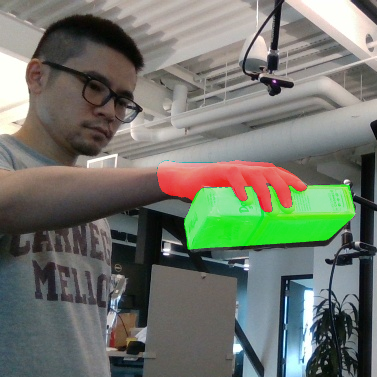
\includegraphics[width=0.98\linewidth]{figs/5319_2}
  \end{subfigure}
    \begin{subfigure}[b]{0.16\linewidth}
    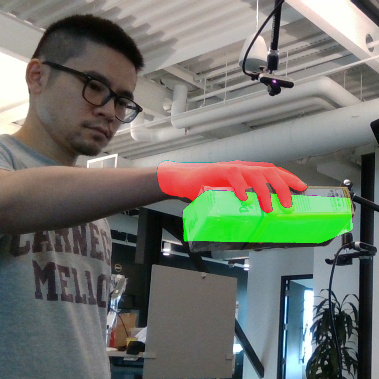
\includegraphics[width=0.98\linewidth]{figs/5319_3}
  \end{subfigure}
    \begin{subfigure}[b]{0.16\linewidth}
    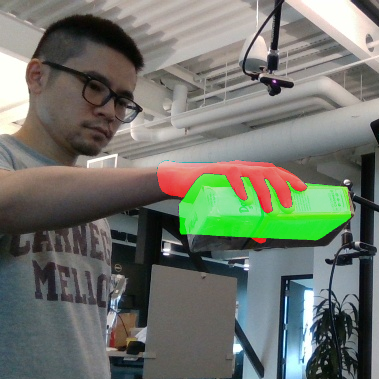
\includegraphics[width=0.98\linewidth]{figs/5319_4}
  \end{subfigure}  
  \vspace{0.2cm}
  
    \begin{subfigure}[b]{0.16\linewidth}
    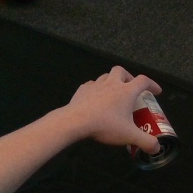
\includegraphics[width=0.98\linewidth]{figs/9063_rgb}
  \end{subfigure}
  \begin{subfigure}[b]{0.16\linewidth}
    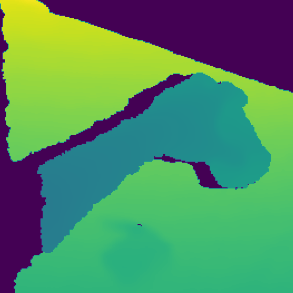
\includegraphics[width=0.98\linewidth]{figs/9063_depth2}
  \end{subfigure}
  \begin{subfigure}[b]{0.16\linewidth}
    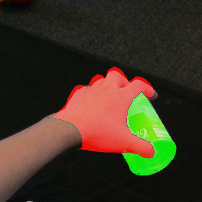
\includegraphics[width=0.98\linewidth]{figs/9063_0}
  \end{subfigure}
  \begin{subfigure}[b]{0.16\linewidth}
    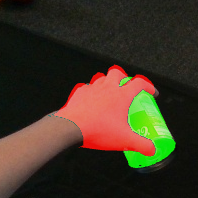
\includegraphics[width=0.98\linewidth]{figs/9063_9}
  \end{subfigure}
    \begin{subfigure}[b]{0.16\linewidth}
    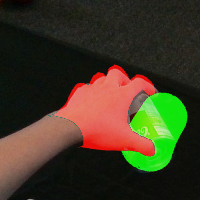
\includegraphics[width=0.98\linewidth]{figs/9063_15}
  \end{subfigure}
    \begin{subfigure}[b]{0.16\linewidth}
    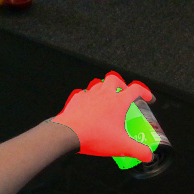
\includegraphics[width=0.98\linewidth]{figs/9063_19}
  \end{subfigure}  
  \vspace{0.2cm}
  
    \begin{subfigure}[b]{0.16\linewidth}
    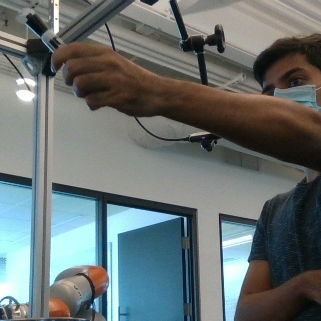
\includegraphics[width=0.98\linewidth]{figs/180000_rgb}
    \caption{RGB}
  \end{subfigure}
  \begin{subfigure}[b]{0.16\linewidth}
    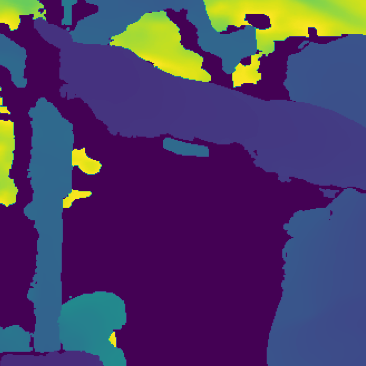
\includegraphics[width=0.98\linewidth]{figs/180000_depth2}
    \caption{Depth}
  \end{subfigure}
  \begin{subfigure}[b]{0.16\linewidth}
    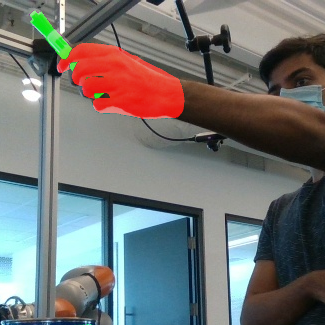
\includegraphics[width=0.98\linewidth]{figs/180000_4}
    \caption{Ground truth}
  \end{subfigure}
  \begin{subfigure}[b]{0.16\linewidth}
    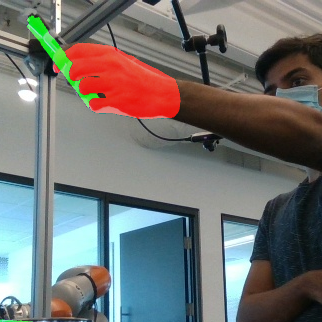
\includegraphics[width=0.98\linewidth]{figs/180000_8}
    \caption{Ours}
  \end{subfigure}
    \begin{subfigure}[b]{0.16\linewidth}
    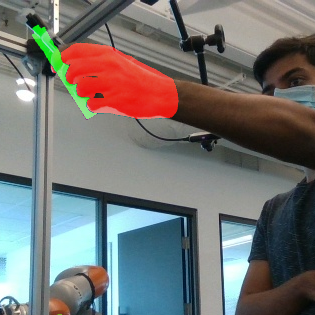
\includegraphics[width=0.98\linewidth]{figs/180000_10}
    \caption{Wang et al. \cite{wang2019densefusion}}
  \end{subfigure}
    \begin{subfigure}[b]{0.16\linewidth}
    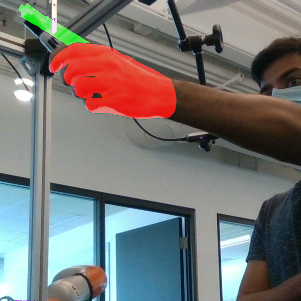
\includegraphics[width=0.98\linewidth]{figs/180000_13}
    \caption{Castro et al. \cite{castro2023crt}}
  \end{subfigure}  
  
  \caption{Qualitative results. (a) and (b) are the input RGBD images. (c) shows the rendered images using ground truth hand and object poses. (d), (e), and (f) display the rendered images using ground truth hand poses and object poses predicted by our method, Wang et al. \cite{wang2019densefusion}, and Castro et al. \cite{castro2023crt}, respectively.}
  \label{fig:result}
\end{figure*}
%--------------------------------------------------

We evaluate our proposed approach on three publicly available datasets: DexYCB \cite{chao2021dexycb}, FPHAB \cite{garcia2018first}, and HO-3D \cite{hampali2020honnotate}. These datasets are chosen for their comprehensive representation of hand-held object interactions, detailed annotations, and diverse scenarios, making them ideal for benchmarking object pose estimation. This evaluation compares our method with state-of-the-art object pose estimation techniques. Furthermore, we assess the impact of our RGB-D fusion module by substituting alternative fusion methods and analyzing the accuracy improvements.

\subsection{Datasets}

\textbf{DexYCB Dataset} (\cite{chao2021dexycb}). This dataset provides 582,000 RGB-D frames across 1,000 sequences with 10 subjects interacting with 20 different objects. Utilizing eight RGB-D cameras, it captures interactions from multiple angles, ensuring rich data diversity. The dataset's precise 3D annotations of both hands and objects make it highly suitable for evaluating hand-held object pose estimation in cluttered environments.

\textbf{FPHAB Dataset} (\cite{garcia2018first}). With over 100,000 frames, this dataset features 45 hand-object interaction categories involving 26 objects. Collected using a motion capture system, it offers detailed 3D annotations, crucial for testing pose estimation models under diverse hand configurations and object manipulations. This diversity aids in assessing the robustness of pose estimation techniques in realistic scenarios.

\textbf{HO-3D Dataset} (\cite{hampali2020honnotate}). Comprising 77,558 frames across 68 sequences, this dataset focuses on challenging hand-object interactions with significant occlusions. It includes RGB images with detailed 3D annotations of hand-object poses, enabling the evaluation of pose estimation methods in complex scenarios. The dataset's challenging conditions test the effectiveness of our approach in real-world applications.

\subsection{\textbf{Implementation Details.}}

All images from each dataset are cropped and resized to $256 \times 256$ pixels. Our implementation\footnote{Our code and other materials are available at \url{https://github.com/hoangcuongbk80/6d_object_inhand}} uses a pre-trained ResNet34 model, originally trained on ImageNet, as the encoder for RGB images. For point cloud feature extraction, we randomly sample 12,288 points from depth images and use a PointNet++-based feature learning network \cite{qi2017pointnet++}, which includes 4 set abstraction (SA) layers and 2 feature propagation (FP) layers. The entire system is implemented using PyTorch and Python, running on an NVIDIA RTX-3090 GPU with an Intel Xeon CPU (12 cores, 2.1GHz), utilizing CUDA and the Linux operating system. For all datasets, we use the Adam optimizer with an initial learning rate of 0.01. The learning rate decays by 0.1 at epochs 80, 140, and 200. We train the model with a batch size of 8 and apply standard data augmentation techniques.

\subsection{Evaluation metric}
\label{sec:metric}

To assess the accuracy of the estimated pose $\hat{P}$ relative to the ground-truth pose $\bar{P}$ of an object model $M$, we use the widely adopted Average Distance of Model Points (ADD) metric \cite{hinterstoisser2012model}. This metric calculates the average distance between corresponding vertices of the object model in the ground-truth pose and the estimated pose. Formally, given the ground truth rotation $\bar{R}$ and translation $\bar{t}$, and the estimated rotation $\hat{R}$ and translation $\hat{t}$, the ADD is defined as:

%----------------------------------------------
\begin{align}
\  ADD = \dfrac{1}{m} \sum_{x \in M} \parallel (\bar{R}x+ \bar{t} - \hat{R}x+ \hat{t}) \parallel
\end{align}
%%%%%%%%%%%%%%%%%%%%%%%%%%%%%%%%%%%%%%%%%%%%%%%%%%%%%%%%%%%%%%%%%%%

\noindent where $m$ is the number of model points. For symmetric objects, we adapt the metric by computing the average distance using the closest point distance method, as in \cite{bregier2017symmetry}. We evaluate the prediction accuracy using average precision ($AP$) \cite{bregier2017symmetry}. A 6D pose estimate is classified as a true positive if the average distance is less than 10\% of the diameter of the smallest bounding sphere of the object. Additionally, we report the area under the $ADD$ curve ($AUC$) \cite{wang2019densefusion}, providing a measure of pose estimation performance across varying thresholds.

\subsection{Results}

%-------------------------------------------------
\begin{table}[h]
\caption{Quantitative results on the DexYCB \cite{chao2021dexycb}, FPHAB \cite{garcia2018first}, and HO-3D \cite{hampali2020honnotate} datasets without Iterative Refinement. Depth-based methods \cite{wang20216d, gao20206d, guo2021efficient}, RGB methods \cite{billings2019silhonet, peng2019pvnet, wang2021gdr, castro2023crt}, and RGBD methods \cite{wang2019densefusion, he2020pvn3d, he2021ffb6d, wu2023geometric, hong2024rdpn6d, lin2024hipose} are compared with our proposed method (Ours).}
\label{tab:dataset_without_ir}
\begin{center}
\begin{tabular}{|l|c|c|c|c|c|c|c|} 
\hline
& \multicolumn{2}{c|}{DexYCB} & \multicolumn{2}{c|}{FPHAB} & \multicolumn{2}{c|}{HO-3D} & Time \\
\hline
Method & $AUC$ & $AP$ & $AUC$ & $AP$ & $AUC$ & $AP$ & $ms$ \\  
\hline 
\cite{wang20216d} & 52.3 & 53.4 & 54.2 & 55.1 & 53.6 & 54.7 & 42 \\
\cite{gao20206d} & 55.4 & 56.1 & 57.3 & 58.2 & 56.7 & 57.6 & 36 \\
\cite{guo2021efficient} & 57.1 & 58.0 & 59.0 & 59.9 & 58.4 & 59.3 & 33 \\
\hline 
\cite{billings2019silhonet} & 54.3 & 55.5 & 56.2 & 57.1 & 55.6 & 56.9 & 35 \\
\cite{peng2019pvnet} & 57.2 & 58.1 & 59.1 & 60.0 & 58.5 & 59.4 & 38 \\
\cite{wang2021gdr} & 59.6 & 60.5 & 61.5 & 62.4 & 60.9 & 61.8 & 32 \\
\cite{castro2023crt} & 61.2 & 62.1 & 63.1 & 64.0 & 62.5 & 63.4 & 30 \\
\hline
\cite{wang2019densefusion} & 60.3 & 61.1 & 62.2 & 63.1 & 61.6 & 62.5 & 42 \\
\cite{he2020pvn3d} & 62.1 & 63.0 & 64.1 & 65.0 & 63.5 & 64.4 & 49 \\
\cite{he2021ffb6d} & 63.4 & 64.2 & 65.3 & 66.2 & 64.8 & 65.7 & 51 \\
\cite{wu2023geometric} & 65.0 & 65.8 & 66.9 & 67.8 & 66.4 & 67.3 & 46 \\
\cite{hong2024rdpn6d} & 66.3 & 67.1 & 68.2 & 69.1 & 67.6 & 68.5 & 55 \\
\cite{lin2024hipose} & 67.5 & 68.4 & 69.6 & 70.5 & 68.9 & 69.8 & 65 \\
Ours & \textbf{80.3} & \textbf{81.2} & \textbf{82.1} & \textbf{83.4} & \textbf{81.5} & \textbf{82.6} & 40 \\
\hline
\end{tabular}
\end{center}
\end{table}
%-------------------------------------------------

\begin{table}[h]
\caption{Quantitative results on the DexYCB \cite{chao2021dexycb}, FPHAB \cite{garcia2018first}, and HO-3D \cite{hampali2020honnotate} datasets with Iterative Refinement.}
\label{tab:dataset_with_ir}
\begin{center}
\begin{tabular}{|l|c|c|c|c|c|c|c|} 
\hline
& \multicolumn{2}{c|}{DexYCB} & \multicolumn{2}{c|}{FPHAB} & \multicolumn{2}{c|}{HO-3D} & Time \\
\hline
Method & $AUC$ & $AP$ & $AUC$ & $AP$ & $AUC$ & $AP$ & $ms$ \\  
\hline 
\cite{wang20216d} & 61.5 & 62.4 & 63.2 & 64.1 & 62.7 & 63.6 & 163 \\
\cite{gao20206d} & 63.2 & 64.0 & 65.1 & 66.0 & 64.5 & 65.3 & 187 \\
\cite{guo2021efficient} & 64.9 & 65.7 & 66.6 & 67.5 & 66.0 & 66.9 & 165 \\
\hline 
\cite{billings2019silhonet} & 62.8 & 63.7 & 64.6 & 65.5 & 63.9 & 64.8 & 160 \\
\cite{peng2019pvnet} & 65.2 & 66.1 & 67.1 & 68.0 & 66.5 & 67.4 & 170 \\
\cite{wang2021gdr} & 66.9 & 67.8 & 68.7 & 69.6 & 68.2 & 69.1 & 185 \\
\cite{castro2023crt} & 68.3 & 69.2 & 70.2 & 71.1 & 69.6 & 70.5 & 178 \\
\hline
\cite{wang2019densefusion} & 67.0 & 67.8 & 68.8 & 69.7 & 68.3 & 69.1 & 240 \\
\cite{he2020pvn3d} & 68.5 & 69.4 & 70.4 & 71.3 & 69.9 & 70.7 & 270 \\
\cite{he2021ffb6d} & 69.8 & 70.7 & 71.7 & 72.6 & 71.2 & 72.0 & 288 \\
\cite{wu2023geometric} & 71.2 & 72.1 & 73.1 & 74.0 & 72.6 & 73.4 & 215 \\
\cite{hong2024rdpn6d} & 72.3 & 73.2 & 74.2 & 75.1 & 73.7 & 74.5 & 265 \\
\cite{lin2024hipose} & 73.5 & 74.4 & 75.4 & 76.3 & 74.9 & 75.7 & 290 \\
Ours & \textbf{86.7} & \textbf{87.2} & \textbf{88.0} & \textbf{88.5} & \textbf{88.3} & \textbf{87.7} & 200 \\
\hline
\end{tabular}
\end{center}
\end{table}

%-------------------------------------------------

Table \ref{tab:dataset_without_ir} and \ref{tab:dataset_with_ir} present the quantitative results, while Figure \ref{fig:result} illustrates the qualitative results. The proposed method achieves the highest accuracy across all datasets (DexYCB \cite{chao2021dexycb}, FPHAB \cite{garcia2018first}, HO-3D \cite{hampali2020honnotate}) in both AUC and AP metrics. For instance, in the DexYCB dataset, our method achieves an AUC of 80.3 and an AP of 81.2 without iterative refinement, and an AUC of 86.7 and an AP of 87.2 with iterative refinement. The results indicate that RGBD-based methods generally outperform RGB-only \cite{billings2019silhonet, peng2019pvnet, wang2021gdr, castro2023crt} and depth-only methods \cite{wang20216d, gao20206d, guo2021efficient}, leveraging the complementary information from both modalities for superior 3D pose estimation. Among the RGBD methods \cite{wang2019densefusion, he2020pvn3d, he2021ffb6d, wu2023geometric, hong2024rdpn6d, lin2024hipose}, our approach stands out not only for its accuracy but also for its computational efficiency. Despite not being the fastest overall, our method is the fastest among RGBD methods, with a runtime of 40 ms without iterative refinement and 200 ms with iterative refinement, making it feasible for robotic applications. Depth-based methods, such as those by Wang et al. \cite{wang20216d}, Gao et al. \cite{gao20206d}, and Guo et al. \cite{guo2021efficient}, exhibit reasonable speeds but do not achieve the same level of accuracy as RGBD methods. Conversely, RGB methods \cite{billings2019silhonet, peng2019pvnet, wang2021gdr, castro2023crt}, while faster, sacrifice some accuracy compared to RGBD methods. This balance of high accuracy and competitive speed highlights the practical applicability of our method in real-world scenarios.

\subsection{Ablation Study}

%-------------------------------------------------
\begin{table}[h]
\caption{Ablation study without Iterative Refinement. The table compares our full method with versions that exclude hand keypoint voting (w/o hand keypoints), the vote-based fusion module using channel attention (w/o $\mathcal{M}_{fus}$), and hand-aware object pose estimation using self-attention (w/o $\mathcal{M}_{hao}$).}
\label{tab:ablation_without_ir}
\begin{center}
\begin{tabular}{|l|c|c|c|c|c|c|c|} 
\hline
& \multicolumn{2}{c|}{DexYCB} & \multicolumn{2}{c|}{FPHAB} & \multicolumn{2}{c|}{HO-3D} & Time \\
\hline
Method & $AUC$ & $AP$ & $AUC$ & $AP$ & $AUC$ & $AP$ & $ms$ \\  
\hline 
w/o hand keypoints & 76.2 & 77.1 & 76.8 & 79.3 & 75.2 & 77.6 & 38 \\

w/o $\mathcal{M}_{fus}$ & 70.5 & 71.3 & 71.4 & 72.1 & 68.4 & 70.2 & 39 \\

w/o $\mathcal{M}_{hao}$ & 77.8 & 79.2 & 77.5 & 79.7 & 76.3 & 77.8 & 40 \\

Full & \textbf{80.3} & \textbf{81.2} & \textbf{82.1} & \textbf{83.4} & \textbf{81.5} & \textbf{82.6} & 40 \\
\hline
\end{tabular}
\end{center}
\end{table}
%-------------------------------------------------

\begin{table}[h]
\caption{Ablation study with Iterative Refinement.}
\label{tab:ablation_with_ir}
\begin{center}
\begin{tabular}{|l|c|c|c|c|c|c|c|} 
\hline
& \multicolumn{2}{c|}{DexYCB} & \multicolumn{2}{c|}{FPHAB} & \multicolumn{2}{c|}{HO-3D} & Time \\
\hline
Method & $AUC$ & $AP$ & $AUC$ & $AP$ & $AUC$ & $AP$ & $ms$ \\  
\hline 
w/o hand keypoints & 84.2 & 85.1 & 86.1 & 86.5 & 85.2 & 85.0 & 190 \\

w/o $\mathcal{M}_{fus}$ & 75.5 & 75.6 & 76.3 & 76.8 & 75.4 & 75.7 & 268 \\

w/o $\mathcal{M}_{hao}$ & 84.5 & 85.6 & 85.6 & 86.3 & 85.8 & 85.3 & 192 \\

Full & \textbf{86.7} & \textbf{87.2} & \textbf{88.0} & \textbf{88.5} & \textbf{88.3} & \textbf{87.7} & 200 \\
\hline
\end{tabular}
\end{center}
\end{table}
%-------------------------------------------------


The ablation study reveals the significance of each component in our method for RGBD fusion in hand-held object pose estimation (see Table \ref{tab:ablation_without_ir} and \ref{tab:ablation_with_ir}). Removing the hand keypoint voting mechanism resulted in a notable drop in performance across all datasets and metrics. For instance, without hand keypoints, the AUC decreased from 80.3 to 76.2 on DexYCB, 82.1 to 76.8 on FPHAB, and 81.5 to 75.2 on HO-3D. This highlights the critical role of hand keypoint voting in enhancing the accuracy of pose estimation by providing valuable spatial cues. The exclusion of the vote-based fusion module using channel attention ($\mathcal{M}_{fus}$) led to the most significant performance drop, with the AUC falling to 70.5, 71.4, and 68.4 on DexYCB, FPHAB, and HO-3D, respectively. This substantial decrease underscores the importance of the vote-based fusion module in effectively combining RGB and depth features, which is crucial for accurate pose predictions. Removing the hand-aware object pose estimation module ($\mathcal{M}_{hao}$) caused a moderate decrease in performance. The AUC dropped to 77.8, 77.5, and 76.3 on DexYCB, FPHAB, and HO-3D, respectively. The self-attention mechanism that learns the relationship between the hand and the object significantly contributes to the overall accuracy of pose estimation, even though it is not as critical as the vote-based fusion module. The full model, incorporating all components, achieved the highest performance across all datasets and metrics, with an AUC of 80.3, 82.1, and 81.5 on DexYCB, FPHAB, and HO-3D, respectively. This confirms the effectiveness of our proposed method and the synergistic benefits of combining hand keypoint voting, vote-based fusion with channel attention, and hand-aware object pose estimation. The computational time for the full model is 40 ms without iterative refinement and 200 ms with iterative refinement, which, despite a slight increase compared to some ablated versions, remains within a reasonable range. These results justify the additional computational cost, making the full model the most robust and accurate for hand-held object pose estimation.

\section{Conclusion}

In this paper, we have introduced a novel deep neural network designed for the 6D pose estimation of hand-held objects using RGB-D images. Our approach tackles the significant challenges posed by occlusions from the hand and the complexities in effectively fusing RGB and depth data.  Our network leverages a voting scheme where both 2D and 3D keypoints cast votes for the object’s pose, significantly enhancing the estimation in scenarios with occluded objects. Additionally, we model the interaction between the hand and the object through a self-attention mechanism, which captures complex spatial relationships and improves the robustness of the pose estimation process. Extensive experiments on three public datasets demonstrate that our method outperforms existing approaches in terms of accuracy and robustness. Our vote-based RGBD fusion framework offers a promising solution for hand-held object pose estimation, particularly in challenging scenarios involving occlusions and complex hand-object interactions. Future work will focus on further improving the efficiency of the model and exploring its application to a broader range of objects and environments. \\

CRediT authorship contribution statement \\
Dinh-Cuong Hoang: Writing – review \& editing, Writing – original draft, Visualization, Validation, Software, Methodology, Funding acquisition, Data curation, Conceptualization. Dinh-Cuong Hoang: Validation, Investigation, Formal analysis, Data curation. Dinh-Cuong Hoang: Writing – review \& editing, Project administration, Funding acquisition, Formal analysis. Dinh-Cuong Hoang: Validation, Supervision, Funding acquisition. \\ 

Declaration of competing interest \\
The authors declare that they have no known competing financial interests or personal relationships that could have appeared to influence the work reported in this paper.

%%%%%%%%%%%%%%%%%%%%%%%%%%%%%%%%%%%%%%%%%%%%%%%%%%%%%%%%%%%%%%%%%%%%%%

% Main text
%\section{Intro}\label{intro}

% Numbered list
% Use the style of numbering in square brackets.
% If nothing is used, default style will be taken.
%\begin{enumerate}[a)]
%\item 
%\item 
%\item 
%\end{enumerate}  

% Unnumbered list
%\begin{itemize}
%\item 
%\item 
%\item 
%\end{itemize}  

% Description list
%\begin{description}
%\item[]
%\item[] 
%\item[] 
%\end{description}  

% Figure
%\begin{figure}[<options>]
%	\centering
%		\includegraphics[<options>]{}
%	  \caption{}\label{fig1}
%\end{figure}


%\begin{table}[<options>]
%\caption{}\label{tbl1}
%\begin{tabular*}{\tblwidth}{@{}LL@{}}
%\toprule
%  &  \\ % Table header row
%\midrule
% & \\
% & \\
%& \\
% & \\
%\bottomrule
%\end{tabular*}
%\end{table}

% Uncomment and use as the case may be
%\begin{theorem} 
%\end{theorem}

% Uncomment and use as the case may be
%\begin{lemma} 
%\end{lemma}

%% The Appendices part is started with the command \appendix;
%% appendix sections are then done as normal sections
%% \appendix

%\section{Method}\label{method}

% To print the credit authorship contribution details
%\printcredits

%% Loading bibliography style file
%\bibliographystyle{model1-num-names}
\bibliographystyle{cas-model2-names}

% Loading bibliography database
\bibliography{cas-refs}

% Biography
%\bio{}
% Here goes the biography details.
%\endbio

%\bio{pic1}
% Here goes the biography details.
%\endbio

\end{document}

